\chapter{Fakult�ten und Binominialkoeffizienten}
%MARK: Chapter 1
\begin{fdefinition}[Fakult�t]
%MARK: Definition 1.1
F�r $n \in \mathbb{N}_0$ definiert man die Fakult�t $n!$ von $n$ durch:
%MA2-18.03.2009-FORM1
\[n! = \begin{cases}
1 \text{ f�r } n = 0\\
(n - 1)! \mal n \text{ f�r } n \grgl 1
\end{cases}\]
\end{fdefinition}

\section{Anwendung der Fakult�t}
\begin{enumerate}
\item Anzahl aller Anordnungen einer Menge von Elementen $N = \gklamm{1, 2, 3, \dots, n}$ ist $n!$\\
		Eine Anordnung einer Menge nennt man auch \indexi{Permutation}\\
		\ac{z.B.} $n = 3$, $N = \gklamm{1, 2, 3}$

		\begin{figure}[h]
		\centering
		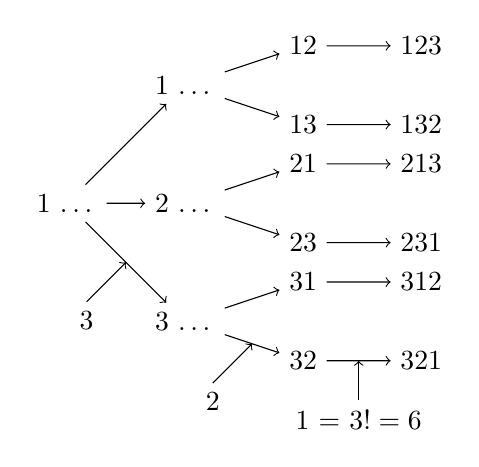
\begin{tikzpicture}[level 2/.style={sibling distance=10mm}]
			\node{1 \dots}[grow=right]
			child[->]{node{3 \dots}
				child[->]{node{32} 
					child[->]{node{321} edge from parent coordinate (desc3)}
				edge from parent 
				coordinate (desc2)}
				child[->]{node{31}
					child[->]{node{312}}}
			edge from parent 
			coordinate (desc1)}
%
			child[->]{node{2 \dots}
				child[->]{node{23}
					child[->]{node{231}}}
				child[->]{node{21}
					child[->]{node{213}}}}
%
			child[->]{node{1 \dots}
				child[->]{node{13}
					child[->]{node{132}}}
				child[->]{node{12}
					child[->]{node{123}}}};

		\draw[->] (desc1) +(-0.5,-0.5) node[below] {3} -- (desc1);
		\draw[->] (desc2) +(-0.5,-0.5) node[below] {2} -- (desc2);
		\draw[->] (desc3) +(0,-0.5) node[below] {1 = $3! = 6$} -- (desc3);
		\end{tikzpicture}
		\Img{MA2-18.03.2009-DIA2}
		\end{figure}

\item Anzahl M�glichkeiten aus einer $n$-\ac{elem.} Grundmenge $N = \gklamm{1, 2, 3, \dots, n}$ eine $k$-\ac{elem.} Teilmenge auszuw�hlen $(k \grgl n)$
		\ac{z.B.} $n = 49$, $k = 6$ (Lotto)\\
		$\text{Anzahl} = \frac{49 \mal 48 \mal 47 \mal 46 \mal 45 \mal 44}{6!} = 13938816 \approx 14 \text{Mio}$\\
		\underline{$n, k$} $\Ra$ $\text{Anzahl} = \frac{n \mal (n - 1) \mal (n - 2) \mal \dots \mal (n - k + 1)}{k!}$\\
\end{enumerate}

\begin{fdefinition}[Binominialkoeffizient]
%MARK: Definition 1.2
F�r $n, k \in \mathbb{N}_0$ und $0 \klgl k \klgl n$ definiert man den \indexu[Binominialkoeffizient]{Binominialkoeffizienten} $\binom{n}{k}$ (''$n$ �ber $k$'' oder ''$n$ tief $k$'') durch
\[\binom{n}{k} = \frac{n!}{k! \mal (n - k)!}\]
\end{fdefinition}

\begin{bemerkung}
\mbox{}\par
\[\frac{n \mal (n - 1) \mal (n - 2) \mal \dots \mal (n - k + 1)}{k!} \mal \frac{(n - k) \mal (n - k - 1) \mal \dots \mal 2 \mal 1}{(n - k) \mal (n - k - 1) \mal \dots \mal 2 \mal 1} = \frac{n!}{k! \mal (n - k)!}\]
\end{bemerkung}

\section{Aufgabe 1.1}
\label{sec:Fakultaet_und_Binominalkoeffizient_A1_1}
%MARK: Aufgabe 1.1
\begin{enumerate}[label=\alph*)]
\item Um von Punkt $0 = (0 \vert 0)$ zum Punkt $P = (6 \vert 4)$ zu gelangen, wollen wir uns nur auf Wegst�cken bewegen, die durch ganzzahlige Gitterpunkte des $\mathbb{R}^2$ gehen und parallel zu einer Koordinatenachse verlaufen.\\
		(Beispiel eines solchen Weges von 0 nach  P)
		\begin{figure}[h]
		\centering
		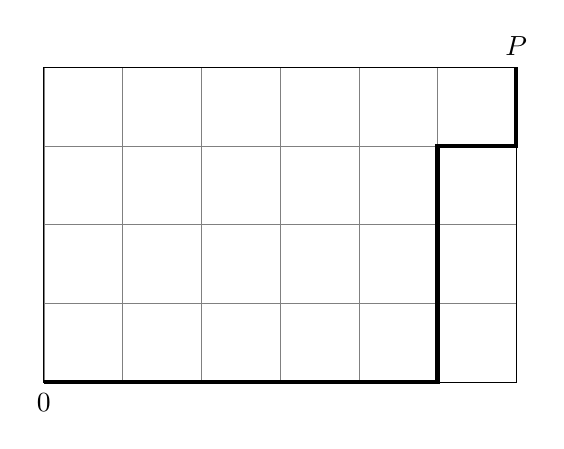
\begin{tikzpicture}
			\draw[step=1,gray,very thin] (0,0) grid (6,4);
			\draw (0,0) rectangle (6,4);
			\draw[ultra thick] (0,0) node[below]{$0$} -- (5,0) -- (5,3) -- (6,3) -- (6,4) node[above]{$P$};
		\end{tikzpicture}
		\end{figure}
		Auf wie vielen Wegen der minimalen L�nge $l = 6 + 4$ kann man von $0$ nach $P$ gelangen? (Vom Gitterpunkt $(i \vert  j)$ bewegt man sich also entweder zum Gitterpunkt $(i + 1 \vert j)$ oder $(i \vert j + 1)$.

\item Wie viele $12$-stellige Zahlen, bei denen die Ziffer $9$ genau zweimal auftritt, lassen sich aus den Ziffern $1, 2, \dots, 9$ bilden?\\
		(Das Produkt muss nicht ausmultipliziert werden.)
\end{enumerate}

L�sung siehe \vref{sec:Fakultaet_und_Binominalkoeffizient_A1_1L}.

\begin{fsatz}[Eigenschaften von Binominialkoeffizienten (Teil 1)]
%MARK: Satz 1.3 Teil 1
\label{satz:Fakultaet_und_Binominalkoeffizient_Satz1_3T1}
Es seien $n, k \in \mb{N}_0$, dann gilt:
\begin{enumerate}[label=\roman*)]
\item $\binom{n}{0} = \binom{n}{n} = 1$
\item $0 \klgl k \klgl n \binom{n}{k} = \binom{n}{n - k}$
\item $0 \klgl k \klgl k \klgl n - 1 \binom{n}{k} + \binom{n}{k + 1} = \binom{n + 1}{k + 1}$
		$\binom{n}{k} + \binom{n}{k + 1} = \frac{n!}{k! (n - k)!} + \frac{n!}{(k + 1)! \mal (n - k - 1)!}$\\
		$= \frac{n!}{k! \mal (n - k)!} \mal \left(\frac{1}{1 \mal (n - k)} + \frac{1}{(k + 1) \mal 1}\right)$\\
		$= \frac{n!}{k! \mal (n - k - 1)!} \mal \frac{k + 1 + n - k}{(n - k) (k + 1)} = \frac{(n + 1)!}{(k + 1)! \mal (n - k)!} = \binom{n + 1}{k + 1}$
\end{enumerate}
\end{fsatz}

\subsection*{Anschauliche Bedeutung von Satz \ref{satz:Fakultaet_und_Binominalkoeffizient_Satz1_3T1}}
F�r i), ii) betrachteten wir eine Menge $\gklamm{1, 2, 3, \dots, n}$
\begin{enumerate}[label=\roman*)]
\item Es gibt nur eine $0$-\ac{elem.} Teilmenge, n�mlich $\emptyset$ also ist $\binom{n}{0} = 1$\\
		Es gibt nur eine $n$-\ac{elem.} Teilmenge n�mlich $\gklamm{1, 2, \dots, n}$, damit $\binom{n}{n} = 1$

\item Wenn wir aus der Menge $\gklamm{1, 2, \dots, n}$ eine $k$-\ac{elem.} Teilmenge w�hlen, bleibt eine $n$-$k$-\ac{elem.} Teilmenge �brig.\\
		$n = 5$, $k = 3$ $\gklamm{1, 2, 3, 4 ,5}$
		\begin{table}[h]
		\centering
		\begin{tabular}{ccc}
		3-\ac{elem.} \ac{Teilm.} & & 2-\ac{elem.} \ac{Teilm.}\\
		$\gklamm{1,2,3}$ & $\ral$ & $\gklamm{4,5}$\\
		$\gklamm{1,2,4}$ & $\ral$ & $\gklamm{3,5}$\\
		$\gklamm{1,2,5}$ & $\ral$ & $\gklamm{3,4}$\\
		$\gklamm{1,3,4}$ & $\ral$ & $\gklamm{2,5}$\\
		$\gklamm{1,3,5}$ & $\ral$ & $\gklamm{2,4}$\\
		$\gklamm{1,4,5}$ & $\ral$ & $\gklamm{2,3}$\\
		$\gklamm{2,3,4}$ & $\ral$ & $\gklamm{1,5}$\\
		$\gklamm{2,3,5}$ & $\ral$ & $\gklamm{1,4}$\\
		$\gklamm{2,4,5}$ & $\ral$ & $\gklamm{1,3}$\\
		$\gklamm{3,4,5}$ & $\ral$ & $\gklamm{1,2}$
		\end{tabular}
		\end{table}
		$\binom{5}{3} = \frac{5 \mal 2 \mal 3}{1 \mal 2 \mal 3} = 10 = \binom{5}{2}$

\item Urne mit $n$ wei�en Kugeln mit Nummern $1, 2, \dots, n$ und einer gelben Kugeln mit Nummer $n + 1$.\\
		Wenn man aus dieser Urne $k + 1$ Kugeln zieht, gibt es daf�r $\binom{n + 1}{k + 1}$ M�glichkeiten.
		\begin{description}
		\item[Fall 1:] Gelbe Kugel wird gezogen, damit m�ssen noch $k$ wei�e Kugeln gezogen werden.\\
				\ac{Anz.} M�glichkeiten $\binom{n}{k}$

		\item[Fall 2:] Gelbe Kugel wird \underline{nicht} gezogen, damit m�ssen $k + 1$ wei�e Kugeln gezogen werden \ac{Anz.} M�glichkeiten $\binom{n}{k + 1}$
		\end{description}
		da Fall 1 und 2 nicht gleichzeitig auftreten ist die totale Anzahl $\binom{n}{k} + \binom{n}{k + 1} = \binom{n + 1}{k + 1}$
\end{enumerate}

\section{Pascalsches Dreieck}
Mit Hilfe von $\binom{n}{0} = \binom{n}{n} = 1$ und $\binom{n}{k} + \binom{n}{k + 1} = \binom{n + 1}{k + 1}$ kann man den Binominialkoeffizienten in einem Deiecksschema darstellen.\\
Die im Inneren liegenden Zahlen sind sind die Summe der jeweils dar�ber liegenden beiden Zahlen.
\begin{figure}[h]
\centering
\begin{tikzpicture}[scale=0.5]
	\foreach{\xa/\xb/\xc}in{0/8/2,-2/6/4,0/6/6,2/6/4,-1/5/10,1/5/10,-4/4/6,0/4/20,4/4/6}{\draw(\xa,\xb)node{\xc};}
	\draw(0,10)node (p1){1};
	\foreach{\xa/\xb}in{-1/1,1/1}{\draw(\xa,9)node(p2){\xb};}
	\foreach{\xa/\xb}in{-2/1,2/1}{\draw(\xa,8)node(p3){\xb};}
	\foreach{\xa/\xb}in{-3/1,-1/3,1/3,3/1}{\draw(\xa,7)node(p4){\xb};}
	\foreach{\xa/\xb}in{-4/1,4/1}{\draw(\xa,6)node(p5){\xb};}
	\foreach{\xa/\xb}in{-5/1,-3/5,3/5,5/1}{\draw(\xa,5)node(p6){\xb};}
	\foreach{\xa/\xb}in{-6/1,-2/15,2/15,6/1}{\draw(\xa,4)node(p7){\xb};}

	\foreach{\xa/\xb/\xc}in{0/10/0,-1/9/1,-2/8/2,-3/7/3,-4/6/4,-5/5/5,-6/4/6}{
		\node(n) at (\xa,\xb){};
		\draw[->] (n.west) +(-2,0) node[left] {$n = \xc$} -- (n.west);}

	\draw[->] (p1.north east) +(1,1) node[above] {$\binom{n}{0}$} -- (p1.north east);
	\draw[->] (p2.north east) +(1,1) node[above] {$\binom{n}{1}$} -- (p2.north east);
	\draw[->] (p3.north east) +(1,1) node[above] {$\binom{n}{2}$} -- (p3.north east);
	\draw[->] (p4.north east) +(1,1) node[above] {$\binom{n}{3}$} -- (p4.north east);
	\draw[->] (p5.north east) +(1,1) node[above] {$\binom{n}{4}$} -- (p5.north east);
	\draw[->] (p6.north east) +(1,1) node[above] {$\binom{n}{5}$} -- (p6.north east);
	\draw[->] (p7.north east) +(1,1) node[above] {$\binom{n}{6}$} -- (p7.north east);
\end{tikzpicture}
\end{figure}
\Img{MA2-19.03.2009-IMG1}

\subsection{Implementierung von Binominialkoeffizienten}
\begin{itemize}
\item falls man \underline{alle} Koeffizienten bis zu einem gegebenen $n$ haben will, erfolgt die Implementierung analog zum Pascalschen Dreieck.
\item falls man \underline{einen} Binominialkoeffizienten $\binom{n}{k}$ haben m�chte.\\
		Implementierung in Maple:
		\begin{lstlisting}
		n := ...; k := ...;
		b := 1:
		for i from 1 to n do
			b := b * (n - 1 + 1)/i;
		end do:
		print (b);
		\end{lstlisting}

		\begin{bemerkung}
		Alle Zwischenresultate $b$ sind $\in \mb{N}$
		\begin{itemize}
		\item $\frac{n}{1} \in \mb{N}$
		\item $\frac{n}{1} \mal \frac{(n - 1}{2} \in \mb{N}$, da entweder $n$ oder $n - 1$ gerade
		\item $\frac{n}{1} \mal \frac{(n - 1}{2} \mal \frac{n - 2}{3}$ da (genau) eine der drei Zahlen $n$, $n -1$, $n - 2$ durch $3$ teilbar
		\end{itemize}
		\end{bemerkung}
\end{itemize}

\begin{fsatz}[Binomischer Lehrsatz (Binomische Formel)]
%MARK: Satz 1.4
\label{satz:Fakultaet_und_Binominalkoeffizient_Satz1_4}
F�r $a, b \in \mb{R}$ und $n \in \mb{N}_0$ gilt:
\[\left(a + b\right)^n = \sum_{k = 0}^n \binom{n}{k} \mal a^{n - k} \mal b^k\]
\end{fsatz}

\begin{fbeweis}[Vollst�ndige Induktion]
\mbox{}\par
%MA2-19.03.2009-BEW2
\begin{description}
\item[(IA)] $n = 0$
		\begin{align*}
			LS &= (a + b)^0 = 1\\
			RS &= \sum_{k = 0}^0 \binom{0}{k} \mal a^{0 - k} \mal b^k = 1 \mal 1 \mal 1 = 1 \Ra \text{Wahr}
		\end{align*}

\item[(IS)] \ac{z.z.}: $\forall n \in \mb{N}_0$
		\[(a + b)^n = \sum_{k = 0}^n \mal a^{n - k} \mal b^k \Ra (a + b)^{n + 1} \binom{n + 1}{k} \mal a^{n + 1 - k} \mal b^k\]
		\begin{align*}
			(a + b)^{n + 1} &= (a + b) \mal (a + b)^n \stackrel{\text{(IV)}}{=} (a + b) \sum_{k = 0}^n \binom{n}{k} \mal a^{n - k} \mal b^k\\
			&= \sum_{k = 0}^n \binom{n}{k} \mal a^{n + 1 - k} \mal b^k + \sum_{k = 0}^n \binom{n}{k} \mal a^{n - k} \mal b^{k + 1}\\
			&= a^{n + 1} + \sum_{k = 0}^n \binom{n}{k} \mal a^{n + 1 - k} \mal b^k + b^{n + 1} + \sum_{k = 0}^n \binom{n}{k} \mal a^{n - k} \mal b^{k + 1}\\
			&= a^{n + 1} + b^{n + 1} + \sum_{k = 0}^n \binom{n}{k} \mal a^{n + 1 - k} \mal b^k + \sum_{\underbrace{k = 0}_{\begin{array}{cc}&l = k + 1\\\Lra & k = l - 1\end{array}}}^n \binom{n}{l - 1}\\
			&= \binom{n + 1}{0} a^{n + 1} + \binom{n + 1}{n + 1} b^{n + 1} + \sum_{k = 1}^n \underbrace{\left(\binom{n}{k} + \binom{n}{k - 1}\right)}_{\binom{n + 1}{k}} \mal a^{n + 1 - k} \mal b^k\\
			&= \sum_{k = 0}^{n + 1} \mal a^{n + 1 - k} \mal b^k
		\end{align*}
\end{description}
\end{fbeweis}

\subsection*{Anschauliche Begr�ndung f�r Satz \ref{satz:Fakultaet_und_Binominalkoeffizient_Satz1_4}}
$(a + b)^n = \underbrace{(a + b)}_{\text{1. Klammer}} \mal \underbrace{(a + b)}_{\text{2. Klammer}} \mal (a + b) \mal \dots \mal \underbrace{(a + b)}_{\text{$n$-te Klammer}}$
\begin{itemize}
\item Summe der Exponenten von $a$ und $b$ muss $n$ sein
\item $\binom{n}{k}$ \ac{Anz.} m�glicher Wahlen von $k$ Klammern aus der ''$b$'' gew�hlt wird.
\end{itemize}

\begin{beispiel}[Absch�tzung von Gr��enordnungen]
$(1,07)^{10} = 1,067$\\
$(1,07)^{10} = \left(1 + \frac{7}{100}\right)^{10} = \sum_{k = 0}^{10} \underbrace{\binom{10}{k} \mal 1^{10 - k} \mal \left(\frac{7}{100}\right)^k}_{\klgl 0} = *$\\
\begin{align*}
* &\klgl \binom{10}{0} \mal 1^{10} \mal \left(\frac{7}{100}\right)^0 + \binom{10}{1} \mal 1^9 \mal \left(\frac{7}{100}\right)^1\\
&= 1 + 0,7 = 1,7\\
* &\klgl 1 + 0,7 + \underbrace{\binom{10}{2}}_{45} \mal 1^8 \mal \underbrace{\left(\frac{7}{100}\right)^2}_{\frac{49}{10000}} \approx 1,7 + \underbrace{\frac{225}{10000}}_{0,225} = 1,925
\end{align*}
\end{beispiel}

\begin{fsatz}[Eigenschaften von Binominialkoeffizienten (Teil 2)]
\label{satz:Fakultaet_und_Binominalkoeffizient_Satz1_3T2}
Teil 1 siehe Satz \vref{satz:Fakultaet_und_Binominalkoeffizient_Satz1_3T1}
\begin{enumerate}[label = \roman*), start=4]
\item $\sum_{k = 0}^n \binom{n}{k} = (1 + 1)^n = 2^n$
\item $\sum_{k = 0}^n (-1)^k \binom{n}{k} = (1 + (-2))^n = 0$\\$n \grgl 1$
\end{enumerate}
%MARK: Satz 1.3 Teil 2
\end{fsatz}

\subsection*{Interpretation von Satz \ref{satz:Fakultaet_und_Binominalkoeffizient_Satz1_3T2} f�r Mengen}
$\binom{n}{k}$ = Anzahl $k$-\ac{elem.} Teilmengen einer $n$-\ac{elem.} Grundmenge\\
\begin{align*}
\Ra \sum_{k = 0}^n \binom{n}{k} &= \text{ Anzahl aller m�glichen Teilmengen einer $n$-\ac{elem.} Grundmenge}\\
&= \text{ Anzahl Elemente der Potenzmenge einer $n$-\ac{elem.} Menge}\\
&= 2^n
\end{align*}
\[\sum_{k = 0}^n (-1)^k \binom{n}{k} = \underbrace{\sum_{k = 0}^n \binom{n}{k}}_{k \text{ gerade}} - \underbrace{\sum_{k = 0}^n \binom{n}{k}}_{k \text{ ungerade}} = 0\]
\begin{itemize}[label=\Ra]
\item Anzahl Teilmengen der $n$-\ac{elem.} Grundmenge, die eine gerade Anzahl an Elementen enth�lt, ist gleich der Anzahl der Teilmengen mit einer ungeraden Anzahl an Elementen.
\end{itemize}

\section{L�sungen}
\subsection{Aufgabe 1.1}
\label{sec:Fakultaet_und_Binominalkoeffizient_A1_1L}
L�sung zu Aufgabe \vref{sec:Fakultaet_und_Binominalkoeffizient_A1_1}.

\begin{enumerate}[label=\alph*)]
\item Es werden 10 Schritte gelaufen, davon 4 vertikal (und 6 horizontal).\\
		Anzahl Pfade = Anzahl M�glichkeiten die 4 Schritte nach oben aus den 10 auszuw�hlen.
		\[= \binom{10}{4} = \frac{10 \mal 9 \mal 8 \mal 7}{4 \mal 3 \mal 2 \mal 1} = 210\]

\item $8^{10}$ = Anzahl der M�glichkeiten an den Stellen ohne 9.\\
		$\binom{12}{2}$ = Anzahl M�glichkeiten die Stellen f�r die 9en auszusuchen.\\
		Die Formel lautet damit wie folgt:
		\[8^{10} \mal \binom{12}{2} \approx 2,95 \mal 10^{10}\]
\end{enumerate}
